\documentclass[letterpaper, 10pt]{article}
\usepackage[margin=0.45in]{geometry}
\usepackage{xifthen}
\usepackage[colorlinks=true,urlcolor=Blue, hidelinks]{hyperref}
\usepackage{graphicx}  % 插图
% \usepackage{cleveref}
\usepackage{newclude}
\usepackage{titlesec}
\usepackage{metalogo}
\usepackage[utf8]{inputenc}
\usepackage[slantfont,boldfont]{xeCJK} % 允许斜体和粗体
\usepackage{kotex}
\usepackage{amsmath, mathrsfs, amsfonts}
\usepackage{tabularray}
\usepackage[dvipsnames]{xcolor}
\usepackage{titling}
\usepackage{titlesec}
\usepackage{minted}
\usepackage{fontawesome5}
\usepackage[customcolors,shade]{hf-tikz}
\usepackage{tkz-euclide}


\usemintedstyle{xcode}

\newminted{tex}{
  gobble=2,
  linenos,
  mathescape,
  numbersep=5pt,
  frame=single,
  baselinestretch=1.2,
  fontsize=\normalsize,
  highlightcolor=yellow!50,
  highlightlines={},
  breaklines,
}
% Macro to allow image links in XeLaTeX
\ifxetex
  \usepackage{letltxmacro}
  \setlength{\XeTeXLinkMargin}{1pt}
  \LetLtxMacro\SavedIncludeGraphics\includegraphics
  \def\includegraphics#1#{% #1 catches optional stuff (star/opt. arg.)
    \IncludeGraphicsAux{#1}%
  }%
  \newcommand*{\IncludeGraphicsAux}[2]{%
    \XeTeXLinkBox{%
      \SavedIncludeGraphics#1{#2}%
    }%
  }%
\fi
%%%%%%%

\definecolor{bg}{RGB}{0.95,0.95,0.95}
\definecolor{mygrey}{RGB}{128,128,128}
\definecolor{myteal}{RGB}{0,128,128}
\definecolor{mypink}{RGB}{250,218,221}


\setmainfont{Noto Sans CJK SC}
% \setmonofont{Monaco} % 英文等宽字体
% \setsansfont{Trebuchet MS} % 英文无衬线字体
\setCJKmainfont{Noto Sans CJK SC}
\setCJKsansfont{Noto Sans CJK SC}
\setCJKmonofont{Noto Sans CJK SC}

\NewTableCommand\myhline{\hline[0.2em,black]}


\let\oldhref\href
\renewcommand{\href}[3][blue]{\oldhref{#2}{\color{#1}{#3}}}


% Link images
\newcommand{\pdf}{
\includegraphics[height=.85em]{png/pdf.png}}
\newcommand{\gh}{
\includegraphics[height=.85em]{png/gh.png}}
\newcommand{\www}{
\includegraphics[height=.85em]{png/www.png}}
\newcommand{\email}{
\includegraphics[height=.85em]{png/email.png}}
\newcommand{\yt}{
\includegraphics[height=.85em]{png/yt.png}}
\newcommand{\gitee}{
\includegraphics[height=.85em]{png/gitee.png}}

% \title{Constructing a Nuclear Reactor Using Only Coconuts}
\author{LcdSe7en}
\date{\today}


% Custom title command.
\renewcommand{\maketitle}{
	\hspace{.25\textwidth}
	\begin{minipage}[t]{.5\textwidth}
    \par{\centering{\Huge  \texttt{\theauthor}}\par}
	\end{minipage}
	\begin{minipage}[t]{.25\textwidth}
   {\footnotesize\hfill{}\color{gray}
     \hfill{}Download this document:

     \hfill{}\href[gray]{https://github.com/lcdse7en/archlinux}{documents.pdf \pdf}

     \hfill{}(Last updated \thedate.)
    }
	\end{minipage}
}


\UseTblrLibrary{counter}
\newcounter{mycnta}
\newcommand{\mycnta}{\stepcounter{mycnta}\arabic{mycnta}}


\titleformat{\section}{\Large\bf\raggedright}{}{1em}{}[{\titlerule[2pt]}]


\begin{document}

\maketitle


\begin{minipage}[t]{.5\linewidth}
\begin{tabular}{rp{.75\linewidth}}
	\baselineskip=20pt
	\email{} :     & \href{2353442022@qq.com}{2353442022@qq.com}\\
	\www{} : &\href{https://texdoc.org/index.html}{https://texdoc.org/index.html}
\end{tabular}
\end{minipage}
\begin{minipage}[t]{.5\linewidth}
\begin{tabular}{rl}
	\gh{} : & \href{https://github.com/lcdse7en}{https://github.com/lcdse7en}\\
	\gitee{} : &\href{https://gitee.com/se7enlcd}{https://gitee.com/se7enlcd}
\end{tabular}
\end{minipage}

\include*{documents/packages-table} % 不分页

\section{minted  \textcolor{green}{\faIcon{github}} \textcolor{blue}{\faIcon{code}} \faIcon{university} \textcolor{cyan}{\faIcon{google-plus}} \faIcon{at}}

\begin{texcode}
  % sudo pip3 install pygments
  % -shell-escape

  \documentclass[letterpaper, 10pt]{article}
  \usepackage{minted}
  \usepackage{xcolor}
  \usepackage{fontawesome5} % \textcolor{green}{\faIcon{github}}

  \usemintedstyle{xcode} % pygmentize -L styles [xcode, github-dark]
  

  % Custom Code Environments
  \newminted{tex}{
    gobble=2,
    linenos,
    mathescape,
    numbersep=5pt,
    frame=single,
    baselinestretch=1.2,
    fontsize=\normalsize, % huge, LARGE, large, normalsize, small, footnotesize, scriptsize, tiny
    highlightcolor=yellow!50,
    highlightlines={1,3},
    bgcolor=bg,
    breaklines,
  }

  \begin{document}

  % \begin{Customcode}
  \begin{minted}[
      encoding=utf8,
      linenos,
      gobble=2,
      mathescape,
      numbersep=5pt,
      frame=single,
      framesep=2mm,
      baselinestretch=1.2,
      fontsize=\large, % huge, LARGE, large, normalsize, small, footnotesize, scriptsize, tiny
      highlightcolor=yellow!50,
      highlightlines={1,3},
      bgcolor=bg,
      breaklines]{tex}
    ...
  \end{minted}
  % \end{Customcode}

  \end{document}
\end{texcode}

\newpage

\section{graphicx \textcolor{green}{\faIcon{github}} \textcolor{blue}{\faIcon{code}} \faIcon{university} \textcolor{cyan}{\faIcon{google-plus}} \faIcon{at}}


\begin{minted}[
  encoding=utf8,
  linenos,
  gobble=2,
  mathescape,
  numbersep=5pt,
  frame=single,
  framesep=2mm,
  baselinestretch=1.2,
  fontsize=\normalsize, % huge, LARGE, large, normalsize, small, footnotesize, scriptsize
  highlightcolor=cyan!50,
  highlightlines={7,12},
  breaklines]{tex}
  \usepackage{graphicx}

  \begin{figure}[hbt!]
  \centering
  \begin{minipage}{0.49\textwidth}
    \centering
    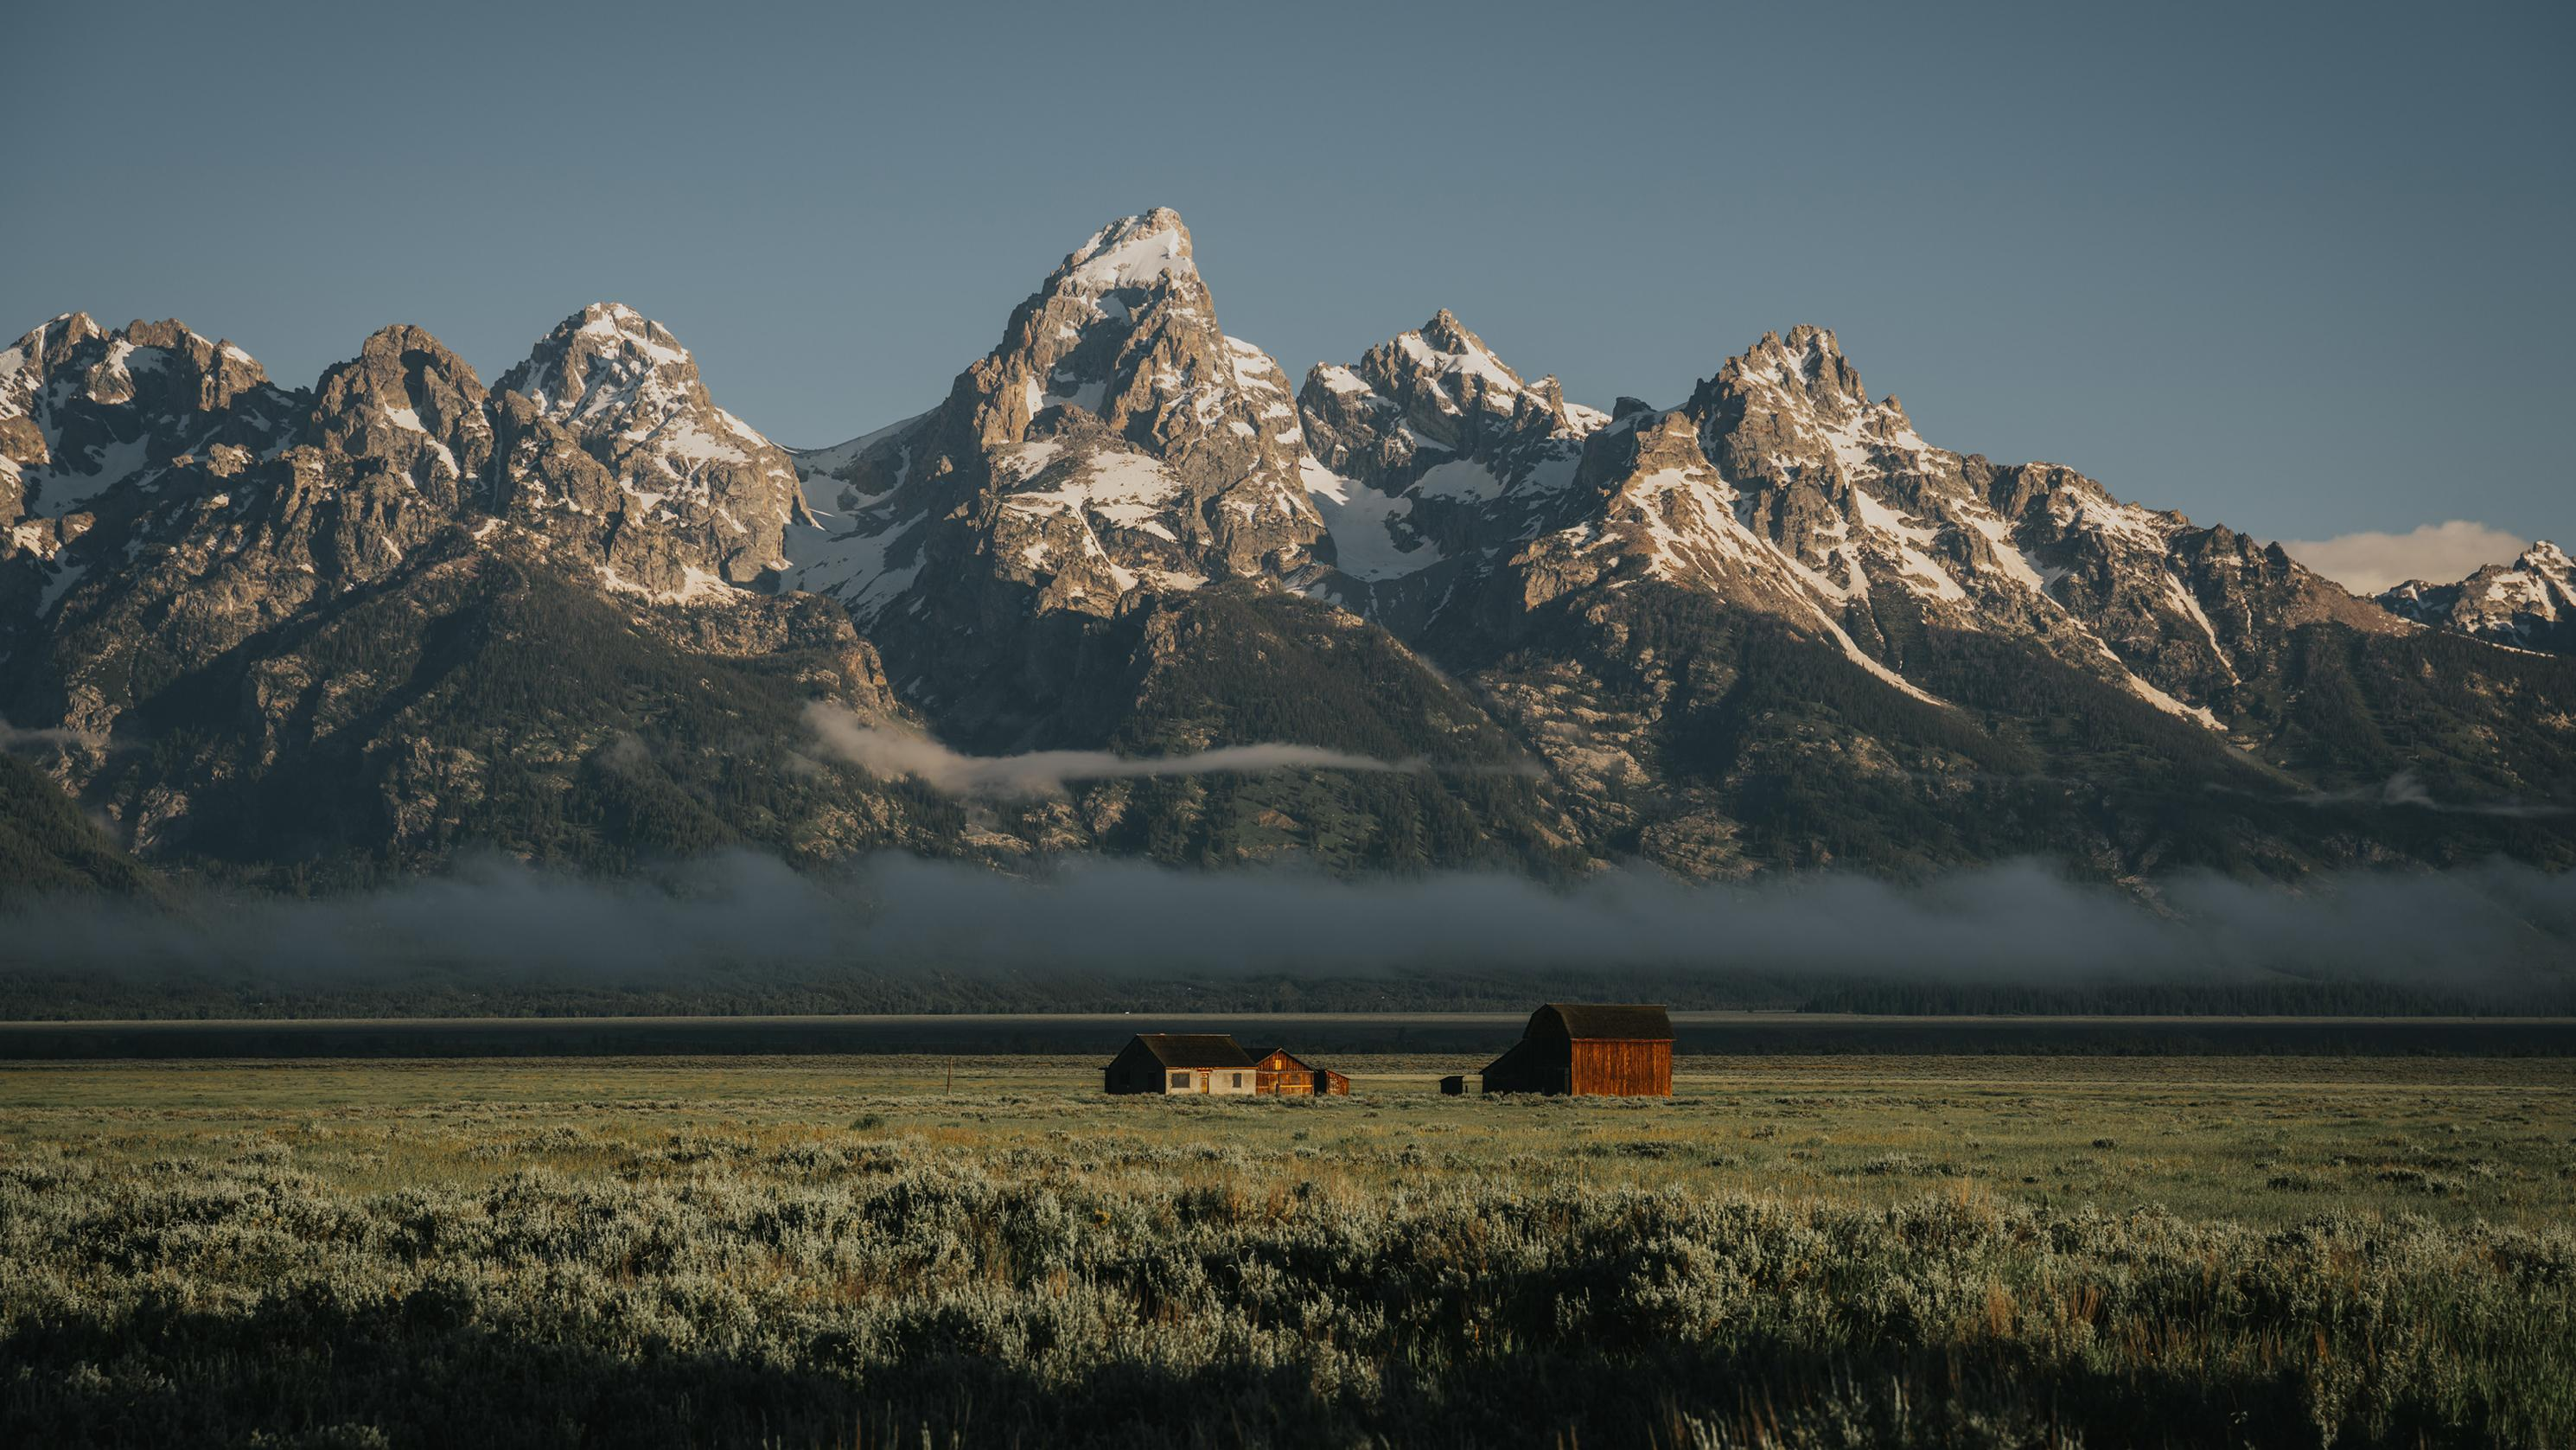
\includegraphics[width=\textwidth]{images/1.jpg}
    \caption{1}
  \end{minipage}
  \begin{minipage}{0.49\textwidth}
    \centering
    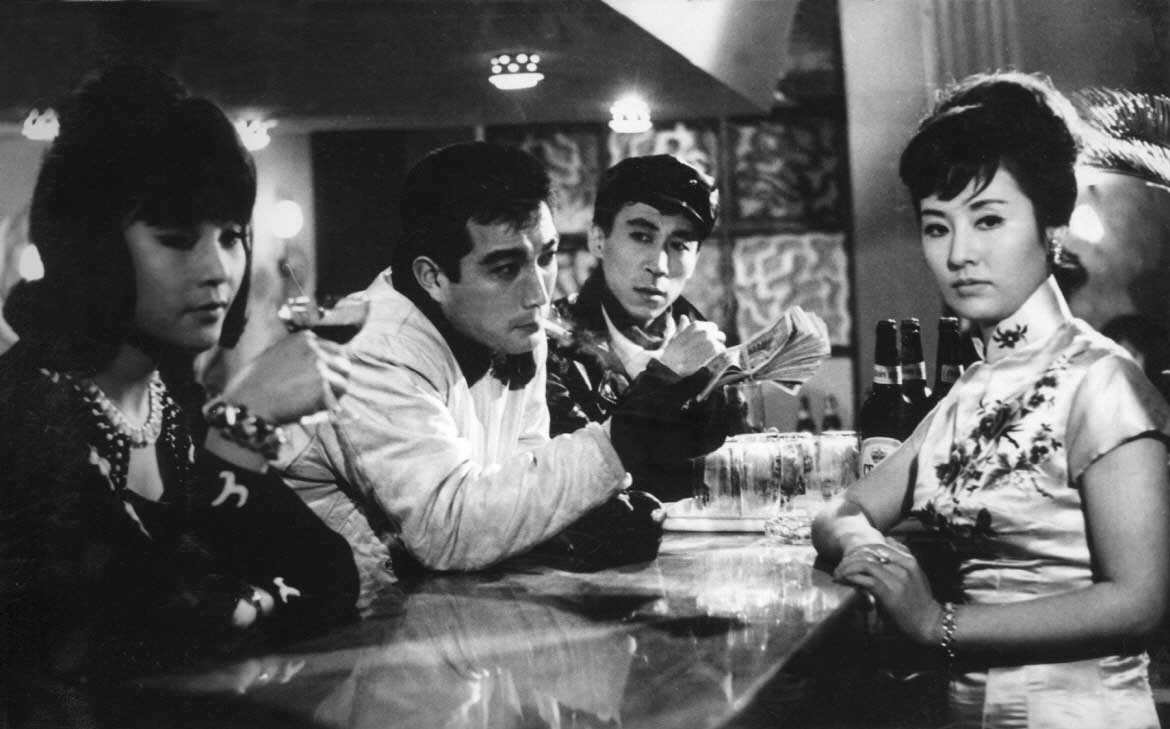
\includegraphics[width=\textwidth]{images/2.jpg}
    \caption{2}
  \end{minipage}
  \end{figure}
\end{minted}


\newpage

% % \begin{minipage}[t][][t]{.6\textwidth}
%   \begin{texcode}
%   \usepackage[customcolors,shade]{hf-tikz}
%   \usepackage{tkz-euclide}

%   \begin{tikzpicture}
%     \tkzDefPoints{0/0/A,4/0/B,3/3/C}
%     \tkzDrawPoints(A,B,C)
%     \tkzLabelPoints(A,B,C)
%     \tkzDrawPolygon(A,B,C) 
%     \tkzLabelSegment[above left](A,C){$\sqrt{13}$}
%     \tkzFillAngle[size=0.5cm, right color=white, left color=red!50](C,B,A)
%     \tkzLabelAngle[pos=1](C,B,A){$26.6^\circ$}
%   \end{tikzpicture}
%   \end{texcode}
% \end{minipage}
% \quad
% \begin{minipage}[t][][b]{.3\textwidth}
%     \begin{tikzpicture}
%       \tkzDefPoints{0/0/A,4/0/B,3/3/C}
%       \tkzDrawPoints(A,B,C)
%       \tkzLabelPoints(A,B,C)
%       \tkzDrawPolygon(A,B,C) 
%       \tkzLabelSegment[above left](A,C){$\sqrt{13}$}
%       \tkzFillAngle[size=0.5cm, right color=white, left color=red!50](C,B,A)
%       \tkzLabelAngle[pos=1](C,B,A){$26.6^\circ$}
%     \end{tikzpicture}
% \end{minipage}

\section{tkz-euclide \textcolor{green}{\faIcon{github}} \textcolor{blue}{\faIcon{code}} \faIcon{university} \textcolor{cyan}{\faIcon{google-plus}} \faIcon{at}}

\begin{tikzpicture}[scale=3]
\tikzset{
arr/.style={postaction=decorate,
decoration={markings,
mark=at position 1 with {\arrow[thick]{#1}}
}}}
\pgfkeys{/pgf/number format/.cd,fixed,precision=2}
\tkzDefPoints{-1/0/A',0/0/A, 1/0/B,2/0/C}
\tkzDefPoints{0/0.5/E,1/0.5/F,2/0.5/G}

\tkzDrawSegment[color=red,thin, arr=stealth](A,C)
\tkzDrawSegment[color=red,thin, arr=stealth](A,E)
\tkzDrawSegment[color=red,thin, arr=stealth](B,F)
\tkzDrawSegment[color=red,thin, arr=stealth](C,G)
\tkzDrawSegment[style=dashed, color=orange](A',A)
\tkzDrawPoints(A',A,B,C)
  \tkzLabelPoints[teal,above left](A)
\tkzDrawLines[add=0 and .5](A,C)
\tkzCalcLength[cm](A,B)\tkzGetLength{ABl}
\tkzCalcLength[cm](B,C)\tkzGetLength{BCl}
% \tkzDrawSegment[dim={\pgfmathprintnumber\ABl,-6pt,transform shape}](A,B)
\tkzDrawSegment[dim={\pgfmathprintnumber\ABl,-6pt,transform shape}](A,B)
\tkzDrawSegment[dim={\pgfmathprintnumber\BCl,-6pt,transform shape}](B,C)
\end{tikzpicture}




\end{document}






